\section{Implementation on Software-defined radio}
\label{sec:real_implementation}

% This part may need to be rearrange.

Two main aspects of measuring the performance of modern communcation systems,
are the latency and throughput. In the previous sections, we focus on explaining and showing
how much accuracy of our proposed joint detection and estimation algorithm can be.
Now in this section, we discuss how to realize our proposed algorithm on software-defined radio (SDR). The algorithm, especially the detection algorithm, should be refined
to fitting very high sample rate since it is applied on every time instant.

\subsection{Modified algorithm in Threading Building Blocks (TBB)}

At the receiver side, in order to make the algorithm work at a very high data rate,
we need to increase the computation efficiency of our detection algorithm as much as possible.
The first improvement is by using pipeline. Threading Building Blocks (TBB) is a well-known C++
library that enables parallel programming on multi-core processors~\cite{TBB_website,TBB_book}.
The Flow Graph interfaces in TBB~\cite[Ch.~3]{TBB_book} can make the algorithm implemented in a simple structure 
and realize pipeline very well by seperating the algorithm into small blocks (nodes), which is used in this paper. 

Figure~\ref{fig:SDR_receiver} illustrates the implementation of the proposed joint detection and estimation algorithm 
in flow graph of TBB. Each block corresponds to a function node in the flow graph.
The received data stream is first buffered into small size of pieces.
The size of buffer should be determined to balance the latency and throughput: an oversized buffer will
cause a long latency while an undersized buffer incurs a large amount of overhead.
Then, the data in buffer is processed for preparing the elements of building the GLRT detector,
which denotes the dashed area. Now, we will go deep explaining the nodes in this area.
The top level generates the SD estimators in a vector in terms of each discrete time instant.
Specifically, the computation of $\hat{\delta}_{\text{SD}}$ in~\eqref{eq:delta_SD} is seperated into 3 steps (nodes):
the first node includes a shift register and calculates the autocorrelation between received samples with sample distance $k$.
The function of shift register is to store the last fraction of received samples in the previous buffer for processing in the current buffer thus
avoid missing detection. The subsequent node calculates the argument in~\eqref{eq:delta_SD}.
Note, the argument can be intepreted as the convolution between autocorrelation vectors of received samples
and of reference samples (one of them should be reversed). Thus, the argument of~\eqref{eq:delta_SD} can be computed more efficiently by fast fourier transform (FFT).

The middle level of the dashed area in Figure~\ref{fig:SDR_receiver} calculates the numerator of phasor estimate for SD estimator in~\eqref{eq:opt_S}.
Compared with the expression of argument in~\eqref{eq:delta_SD}, the numerator of~\eqref{eq:opt_S} performs a time-varing convolution, which cannot be computed
by FFT. However, we can still simiplify the computation by applying functional parallelism in flow graph. 
Figure~\ref{fig:SDR_phasor_SD} illustrates the details of improving the computation in~\eqref{eq:opt_S}. 
$\hat{S}^{\text{(num)}}$ is now computed in two stages: The inner stage has $L_1$ parallel sub nodes each with a shift register in the size of
$N/L_1$; the $L_1$ number of nodes equally seperate the received sequence and calculate the partial dot product
between received samples and the preamble. The outer stage has $L_2$ parallel functional nodes, each corrects the number of $L_1/L_2$ results
from inner stage by frequency estimate at the middle position of the corresponding vector in the inner stage.
Then, $\hat{S}^{\text{(num)}}$ is approximated by adding all the results from outer stages, which yields

\begin{equation}
  \label{eq:refined_opt_S}
  \hat{S}^{\text{(num)}} \approx \sum_{i=0}^{L_2-1} \sum_{m=iL_1/L_2}^{(i+1)L_1/L_2-1} e^{-j\pi \hat{\delta}\frac{N(2m+1)}{L_1}}
  \sum_{n=mN/L_1}^{(m+1)N/L_1-1}r_ns_n^*.
\end{equation}
The accuracy of~\eqref{eq:refined_opt_S} depends on the number of $L_1$ stages. On the other hand,
$L_1$ also determines the number of threads of Central processing unit (CPU) that will be used when running the program.
Thus, the value of $L_1$ should be determined reasonably. 
Moreover, to get a good approximation of $\hat{S}^{\text{(num)}}$, the value of $L_2$ should be the factor of $L_1$.
In conclusion, the combination of the two stages lets the computation of 
$\hat{S}^{\text{(num)}}$ achieving an approximate of $L_1\cdot L_2$ speed up.

\subsection{Signal Transmission Path}

\begin{figure}[t]
  \centerline{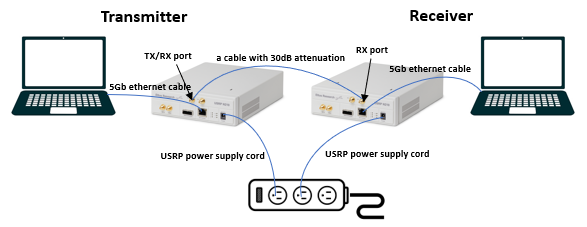
\includegraphics[width=3.4in]{SDR_signal_transmission_path.png}}
  \caption{Machine connection for signal transmission from the transmitter to receiver}
  \label{fig:SDR_signal_transmission_path}
  \end{figure}

In this section, we briefly talk about the signal transmitting path, which is built 
for testing our algorithm. The connection of machines is fairly easy: 
Each of two processors (computers) connected to a universal software radio peripheral (USRP) 
by one 5-Gigabit Ethernet cable as the transmitter or receiver; Between two USRPs,
a cable with~\numb{30}\dB~attenuation connects the RX/TX port and RX port.
At the transmitter side, the processor needs to tell the (transmitter) USRP the sample rate, 
the baseband signal and frequency, the carrier frequency, the transmitter gain, etc. 
Then, the USRP transmits the analog signal to the (receiver) USRP through the two ports.
At the receiver side, the received analog RF signal is first down-converted to baseband, down-sampled to 
discrete-time data stream and finally stored in the local network. After that, our modified algorithm is going to work by requesting the data from the local network.
The outward appearance of the machine connection is shown in Figure~\ref{fig:SDR_signal_transmission_path}.

\subsection{Performance of modified algorithm in TBB}

\begin{table}[t]
  \caption{Benchmark results of function nodes in Figure~\ref{fig:SDR_receiver} (top) and~\ref{fig:SDR_phasor_SD} (bottom)}  % title of Table
  \centering % used for centering table
  \begin{tabular}{c c c c} % centered columns (4 columns)
  \hline\hline %inserts double horizontal lines
  Node name & Time(ns) & CPU(ns) & Iterations \\ [0.5ex] % inserts table
  %heading
  \hline % inserts single horizontal line
  Buffer  & 408721 & 407754 & 1703 \\ % inserting body of the table
  AutoC\_rx (dashed, top left 1) & 160069 & 160054 & 3416 \\
  C\_ctxcrx (dashed, top left 2) & 498967 & 498876 & 1471 \\
  Freq\_SD (dashed, top right 1) & 187135 & 187121 & 3602 \\
  Norm\_rx (dashed, bottom) & 203907 & 203892 & 3416 \\ % [1ex] adds vertical space
  Rho\_p (after dashed area, 1th) & 837253 & 837048 & 829 \\
  Dect (after dashed area, 2nd) & 378793 & 378765 & 1844 \\
  Carrier\_sync (the last) & 811747 & 811739 & 844  \\ [1ex]

  \hline %inserts single line
  C\_rxtx (left column) & 403201 & 403171 & 1736 \\ % inserting body of the table
  Sub\_phasor (right column) & 780620 & 780523 & 886 \\ [1ex]
  \hline
  \end{tabular}
  \label{table:BM_function_nodes} % is used to refer this table in the text
\end{table}
  

To measure the performance of modified algorithm in TBB, we need to consider 
three factors comprehensively: accuracy, throughput and latency. Thus, some parameters should be
chosen by the following rules. First, the length of preamble should be chosen short to get the largest throughput
without degrading the detection and estimation accuracy. Second, the buffer size should be chosen as the power of 2
to achieve the best performance of FFT; Moreover, as discussed, the buffer size should also be chosen
to balance between small overhead and short latency. Third, the value of two stages $L_1$ and $L_2$
in phasor estimate should be chosen large to best obtain the functional parallelism
of flow graph.

As tested, such parameters are determined that can achieve a relatively good performance: 
The preamble is chosen with the number of symbols $L_0=64$ and oversampling factor $M=4$.
The buffer size is 8192. The value of two stages are determined $L_1=2L_2=16$.
The specifications of processor that is used for testing the algorithm at the receiver side are given as follows:
The CPU is Intel(R) Core(TM) i7-9750H, which includes 6 cores and 12 threads.
The best clock speed of CPU can go up to 4500 MHz. Based on above, 
the google benchmark~\cite{Google_benchmark} for each function node in Figure~\ref{fig:SDR_receiver} are shown in Table~\ref{table:BM_function_nodes}.
Note, the time cost in the table should refer to one buffer size, i.e., 8192 received samples; Moreover, the throughput of 
the pipeline is determined by the node with the longest time. Thus, the throughput of the modified algorithm can be ideally approximated by
$8192/837253 \cdot 10^3 \approx 9.78$ MHz.
However, the best throughput cannot go that number because of the limit of maximum clock speed of CPU. 

Based on the above discussion, we test the modified joint detection and estimation algorithm by setting
the sample rate at transmitter be 10 MS/s; Moreover, the transmitter gain plus receiver gain
is 20 dB. As a result, the maximum throughput of the modified algorithm is approaching 4.5 MS/s with latency near 1 ms;
The detection algorithm is very robust and the false alarm probability is near 0.




